\begin{figure}[H]
    \centering
    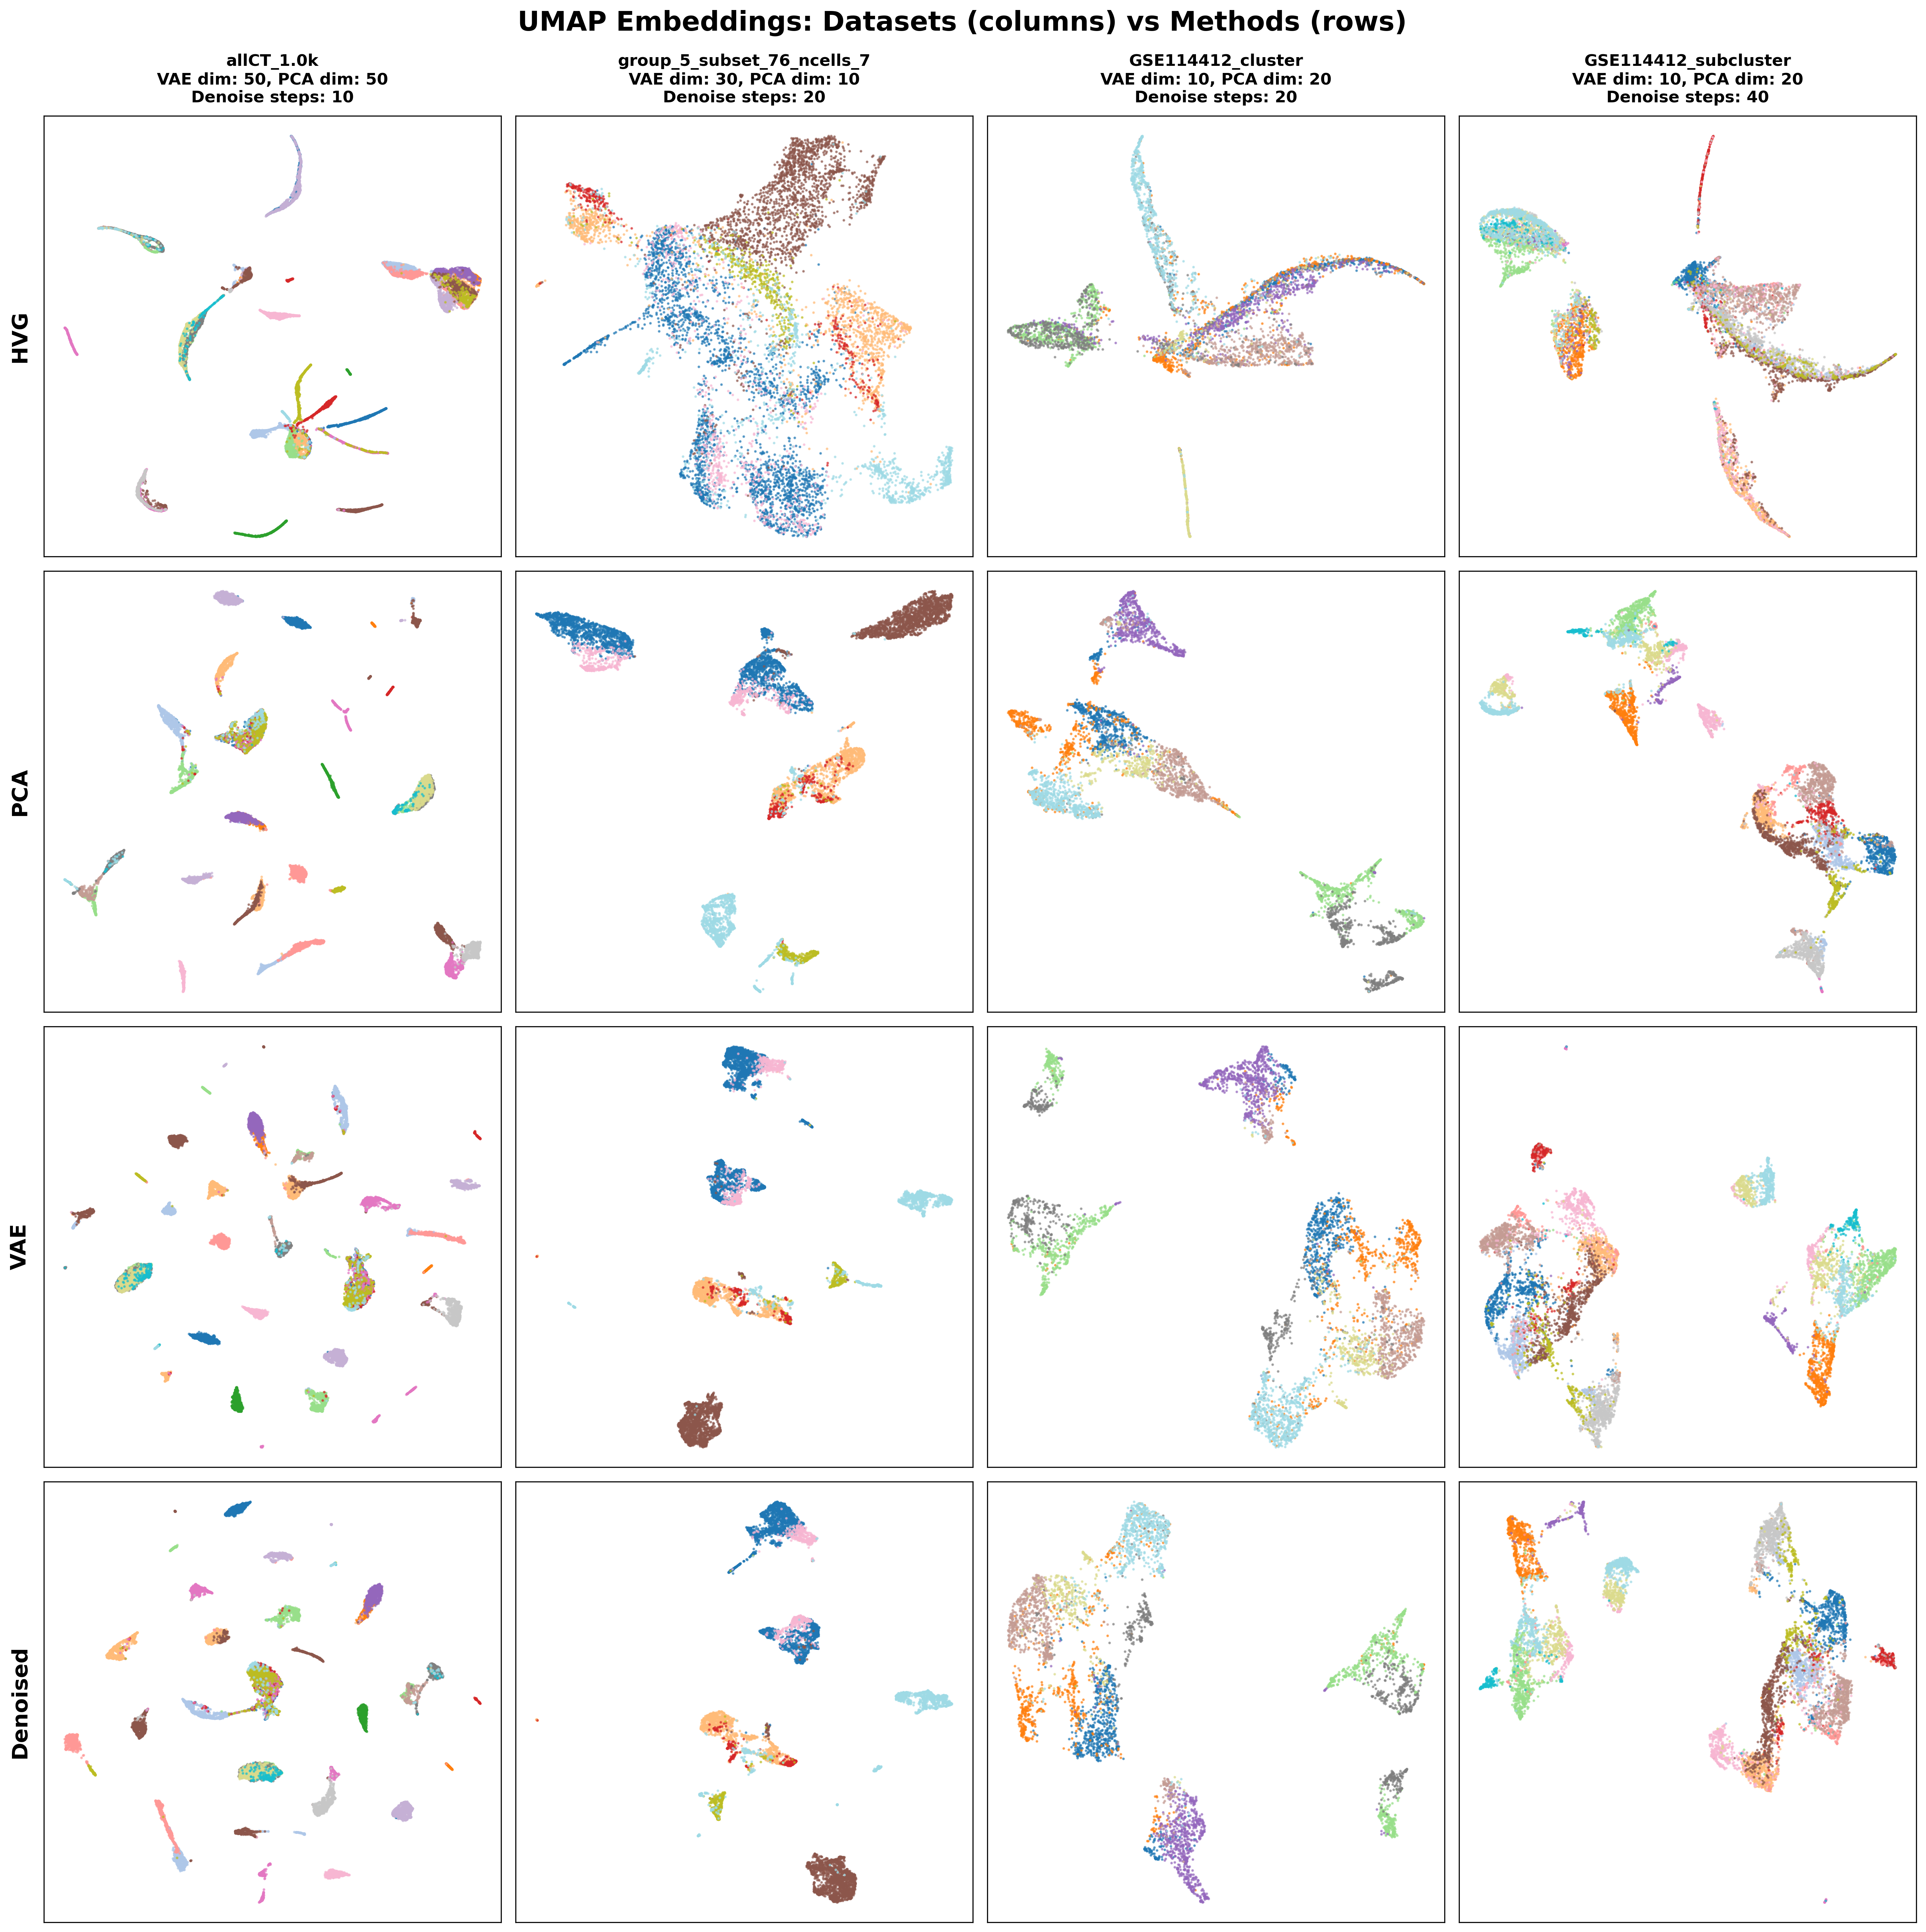
\includegraphics[width=0.9\linewidth]{figures//PART_2_results/umap_comparison_4x4.png}
    \caption{UMAP visualization of embeddings across methods (rows) and datasets (columns). 
    \textbf{Rows:} HVG (raw highly variable genes), PCA, VAE, and Denoised (VAE + LDM). 
    \textbf{Columns:} allCT\_1.0k, group\_5\_subset\_76, GSE114412\_cluster, GSE114412\_subcluster. 
    Points colored by cell type. Dataset-specific hyperparameters (VAE latent dimension, PCA dimension, denoising steps) shown in column headers.}
    \label{fig:umap4x4}
\end{figure}